\section{Ergebnisse}

\subsection{Wirkung des Finetunings}
\label{sec:finetuning-wirkung}

Die erste Forschungsfrage betrifft den Nutzen des Finetunings gegenüber einem unverändert übernommenen vortrainierten Modell. Die Vorgängerarbeit \cite{pagel2025railway} hat auf denselben Aufnahmen mehrere ausschließlich vortrainierte Modelle ohne Anpassung an die Zielszene ausgewertet. Abbildung~\ref{fig:finetuning-baseline} stellt diese Werte dem hier erreichten Fold-Mittel gegenüber.

\begin{figure}[H]
\centering
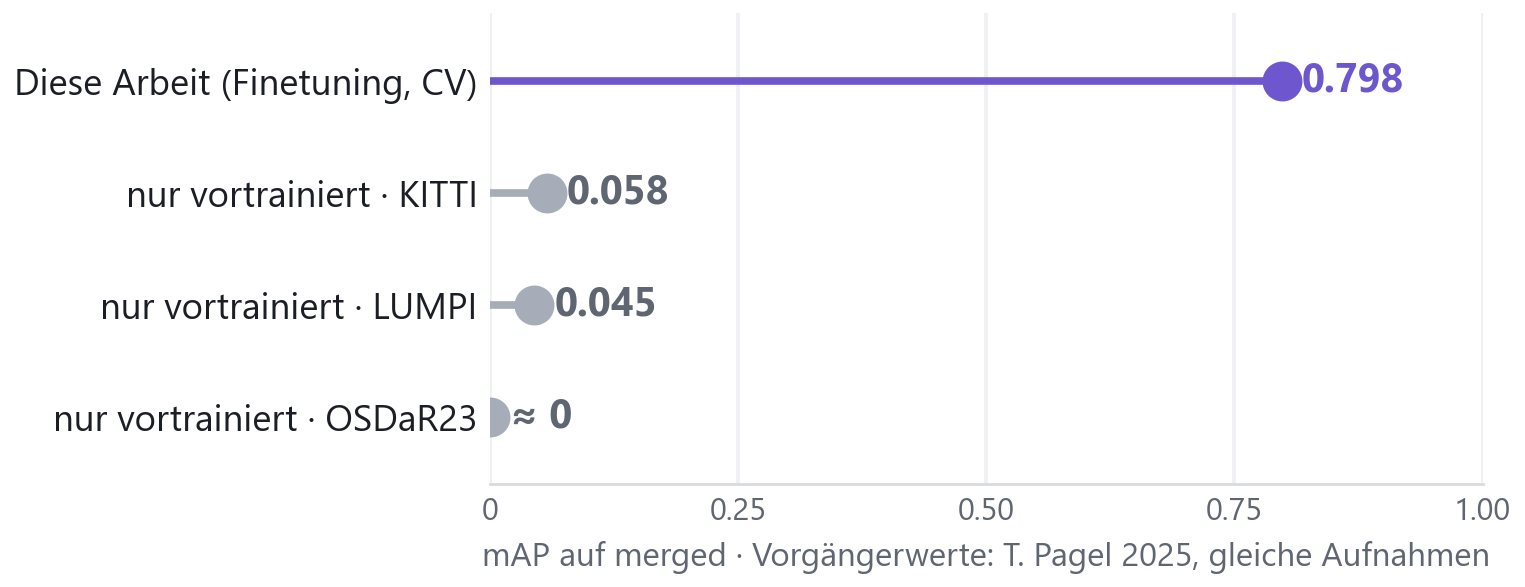
\includegraphics[width=0.9\textwidth]{images/finetuning-baseline.png}
\caption[Finetuning gegenüber vortrainierten Modellen]{Gesamt-mAP auf der fusionierten Ansicht: Finetuning in dieser Arbeit gegenüber ausschließlich vortrainierten Modellen. Die Vergleichswerte stammen aus \cite{pagel2025railway} und wurden auf denselben Tiefgaragenaufnahmen erhoben, aus denen auch Abbildung~\ref{fig:setup} übernommen ist; der Titel jener Arbeit verweist auf einen weiteren, hier nicht betrachteten Anwendungsfall.}
\label{fig:finetuning-baseline}
\end{figure}

Ohne Anpassung an die Zielszene bleiben die vortrainierten Modelle bei einem mAP von 0{,}058 (KITTI), 0{,}045 (LUMPI) beziehungsweise nahe null (OSDaR23). Das in dieser Arbeit auf den Projektdaten finetunete PointPillars erreicht 0{,}798. Der Abstand beträgt damit 0{,}740 mAP; das finetunete Modell erreicht einen ungefähr 14-mal so hohen Wert.

Diese Gegenüberstellung ist ausdrücklich ein Größenordnungsvergleich und keine kontrollierte Ablation. Die Vergleichswerte stammen aus einer anderen Arbeit und wurden nicht unter dem hier verwendeten Cross-Validation-Protokoll erhoben; identisch sind lediglich die zugrunde liegenden Aufnahmen. Insbesondere ist nicht bekannt, ob dort dieselbe Datenkonvertierung und dieselbe AP-Berechnung verwendet wurden. Wie folgenreich das sein kann, zeigt Abschnitt~\ref{sec:konvertierung}: Allein der Wechsel von einer frameweisen auf eine datensatzweite Mittelung veränderte den Fahrrad-AP\textsubscript{30} bei identischem Modelloutput von 0{,}24 auf 0{,}94. Der hier genannte Abstand von 0{,}740 mAP ist deshalb keine quantitativ bestimmte Wirkung des Finetunings. Die Richtung der Aussage ist bei einem Unterschied dieser Größe dennoch eindeutig: Ein direkt übernommenes, auf Außenverkehrsdaten vortrainiertes Netz ist auf dieser Tiefgaragenszene praktisch unbrauchbar. Der Schritt auf die Zieldaten ist der entscheidende Hebel, nicht die Wahl der Architektur -- ein Befund, den der Architekturvergleich in Abschnitt~\ref{sec:centerpoint-ergebnis} stützt.

\subsection{Gesamtleistung von PointPillars}
\label{sec:gesamtleistung}

\begin{table}[H]
\centering
\begin{tabular}{ccccc}
\toprule
\textbf{Ansicht} & \textbf{Fold 1} & \textbf{Fold 2} & \textbf{Fold 3} & \textbf{Mittel \(\pm\) Std.} \\
\midrule
merged & 0{,}840 & 0{,}786 & 0{,}768 & \(0{,}798 \pm 0{,}037\) \\
os0    & 0{,}793 & 0{,}781 & 0{,}757 & \(0{,}777 \pm 0{,}018\) \\
os1    & 0{,}801 & 0{,}751 & 0{,}759 & \(0{,}770 \pm 0{,}027\) \\
\bottomrule
\end{tabular}
\caption{PointPillars Gesamt-mAP über alle Objekte: Fold-Werte, Mittel und Standardabweichung.}
\label{tab:pp-mAP-overall}
\end{table}

Wie Tabelle~\ref{tab:pp-mAP-overall} zeigt, erzielt \texttt{merged} in jedem Fold den höchsten Gesamt-mAP. Der mittlere Vorsprung beträgt ungefähr 0{,}021 gegenüber \texttt{os0} und 0{,}028 gegenüber \texttt{os1}. Bei nur drei Folds ist das kein starker Signifikanznachweis. Es ist jedoch ein konsistenter Hinweis darauf, dass Fusion die ausgewogenste Gesamtleistung liefert und in keinem Fold von einer Einzelsicht übertroffen wird.

Dieser Wert umfasst alle annotierten Objekte, also auch die zahlreichen geparkten Fahrzeuge, die über viele Aufnahmen hinweg an denselben Positionen stehen. Der Gesamt-mAP bewertet damit zwei verschiedene Fähigkeiten zugleich: die Generalisierung auf bewegte Zielobjekte und die Wiedererkennung statischer Szenenbestandteile. Wie stark sich der zweite Anteil auf die einzelnen Ansichten auswirkt, lässt sich aus den vorliegenden Zahlen nicht auftrennen, da die AP keine mengengewichtete Mittelung ist und der statische Anteil sich deshalb nicht herausrechnen lässt. Der folgende Abschnitt wertet die bewegten Objekte separat aus; dort fällt der Abstand zwischen den Ansichten deutlich größer aus.

\subsection{Bewegte Objekte: Gesamtbild}
\label{sec:bewegte-gesamt}

Beschränkt man den mAP auf die bewegten Zielobjekte, vergrößert sich der Abstand deutlich (Abbildung~\ref{fig:map-bewegt}):

\begin{figure}[H]
\centering
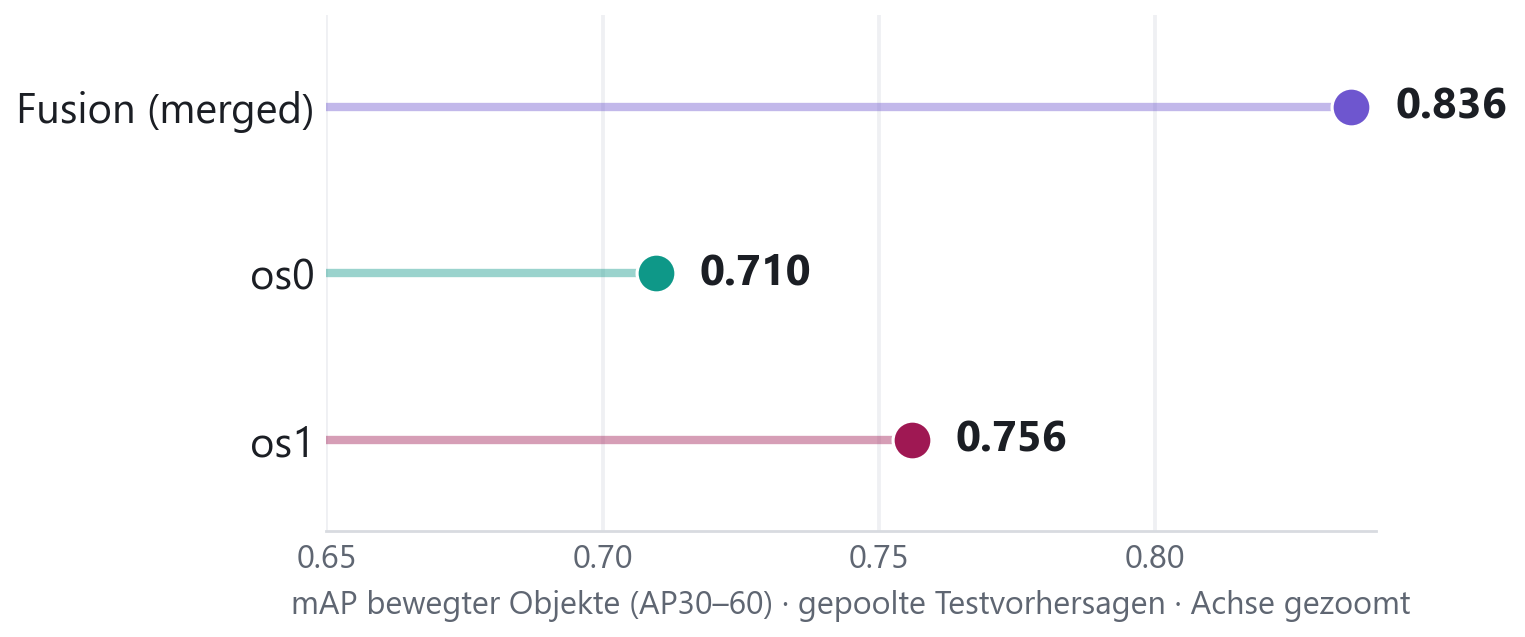
\includegraphics[width=0.9\textwidth]{images/map-bewegte-objekte.png}
\caption[mAP der bewegten Objekte je Ansicht]{mAP über AP\textsubscript{30} bis AP\textsubscript{60} und die drei Klassen, ausschließlich für bewegte Objekte (gepoolte Out-of-Fold-Vorhersagen, labelbasierte Bewegt-/Statisch-Variante).}
\label{fig:map-bewegt}
\end{figure}

Damit der Vergleich mit dem Gesamt-mAP des vorigen Abschnitts nicht zwei verschiedene Schätzer gegenüberstellt, gibt Tabelle~\ref{tab:bewegt-fold} den Bewegt-mAP ebenfalls als Fold-Mittel mit Stichproben-Standardabweichung an, und zwar unter beiden Auswertungsvarianten.

\begin{table}[H]
\centering
\begin{tabular}{cccc}
\toprule
\textbf{Ansicht} & \textbf{alle Objekte} & \textbf{bewegt, offiziell} & \textbf{bewegt, labelbasiert} \\
\midrule
merged & \(0{,}798 \pm 0{,}037\) & \(0{,}784 \pm 0{,}060\) & \(0{,}832 \pm 0{,}038\) \\
os0    & \(0{,}777 \pm 0{,}018\) & \(0{,}736 \pm 0{,}037\) & \(0{,}746 \pm 0{,}031\) \\
os1    & \(0{,}770 \pm 0{,}027\) & \(0{,}744 \pm 0{,}049\) & \(0{,}763 \pm 0{,}049\) \\
\bottomrule
\end{tabular}
\caption{mAP im Fold-Mittel: über alle Objekte sowie ausschließlich über bewegte Objekte, jeweils unter der offiziellen und der labelbasierten Variante.}
\label{tab:bewegt-fold}
\end{table}

Auf einheitlicher Grundlage wächst der Vorsprung der Fusion gegenüber der besseren Einzelansicht von 0{,}021 über alle Objekte auf 0{,}040 in der offiziellen und 0{,}069 in der labelbasierten Bewegt-Auswertung. Die Richtung ist damit in beiden Varianten dieselbe, und der Vergleich ist nun ein Vergleich gleichartiger Schätzer. Die gepoolten Werte in Abbildung~\ref{fig:map-bewegt} liegen mit 0{,}836, 0{,}756 und 0{,}710 nahe an den labelbasierten Fold-Mitteln.

Zwei Beobachtungen ergänzen das Bild. Erstens ist die Fusion in der Bewegt-Auswertung nicht die streuungsärmste Ansicht: Unter der offiziellen Variante liegt ihre Fold-Standardabweichung mit 0{,}060 über der von \texttt{os0} und \texttt{os1}. Zweitens kehrt sich die Reihenfolge der beiden Einzelsensoren um: Über alle Objekte liegt \texttt{os0} vorn, auf den bewegten Objekten \texttt{os1}. Der Unterschied zwischen beiden ist mit 0{,}008 beziehungsweise 0{,}017 allerdings klein gegenüber ihrer Fold-Streuung und sollte nicht als gesicherte Rangfolge gelesen werden.

\subsection{Bewegte Objekte nach Klasse}
\label{sec:bewegte-klassen}

Tabelle~\ref{tab:moving-objects-ap} und Abbildung~\ref{fig:ap30-ap60} schlüsseln dasselbe Ergebnis nach Klasse und IoU-Schwelle auf:

\begin{table}[H]
\centering
{\small\setlength{\tabcolsep}{4pt}
\begin{tabular}{cccc}
\toprule
\textbf{Ansicht} & \textbf{Person AP\textsubscript{30}/AP\textsubscript{60}} & \textbf{Fahrrad AP\textsubscript{30}/AP\textsubscript{60}} & \textbf{Auto AP\textsubscript{30}/AP\textsubscript{60}} \\
\midrule
merged & 0{,}901 / 0{,}729 & 0{,}800 / 0{,}668 & 0{,}891 / 0{,}883 \\
os0    & 0{,}653 / 0{,}370 & 0{,}895 / 0{,}378 & 0{,}885 / 0{,}856 \\
os1    & 0{,}896 / 0{,}426 & 0{,}744 / 0{,}529 & 0{,}832 / 0{,}789 \\
\bottomrule
\end{tabular}}
\caption{Labelbasierte AP\textsubscript{30}/AP\textsubscript{60} für bewegte Objekte nach Ansicht und Klasse (gepoolte OOF-Auswertung).}
\label{tab:moving-objects-ap}
\end{table}

\begin{figure}[H]
\centering
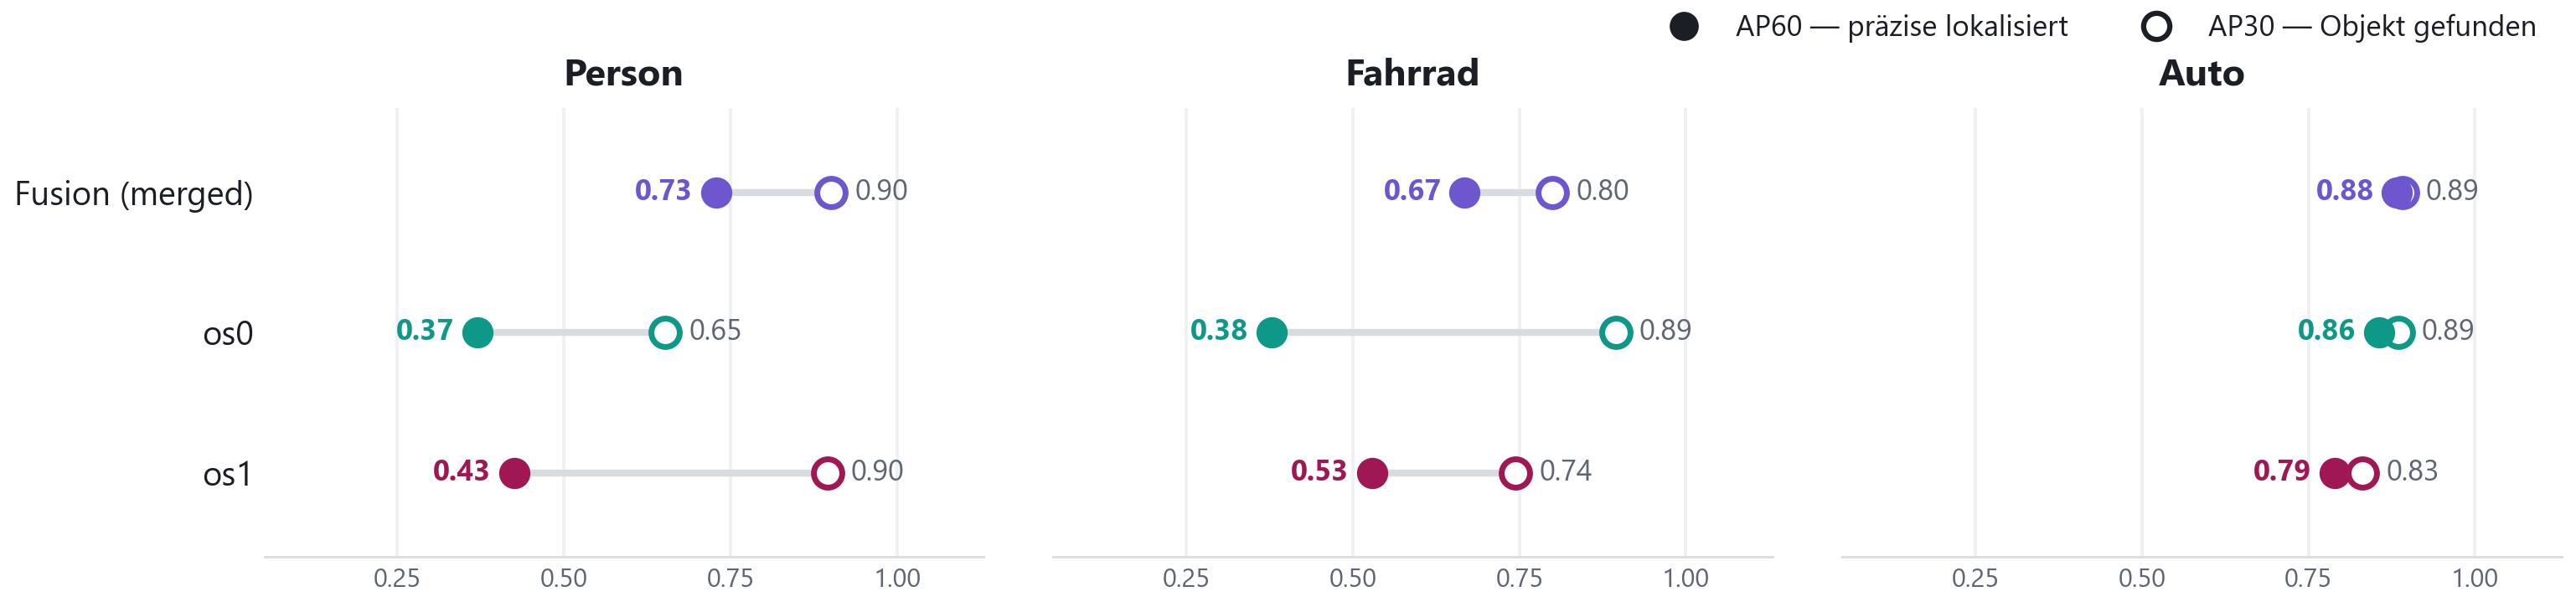
\includegraphics[width=\textwidth]{images/ap30-ap60-klassen.png}
\caption[Detektion gegenüber Lokalisierung je Klasse]{Detektion (AP\textsubscript{30}, offene Ringe) gegenüber präziser Lokalisierung (AP\textsubscript{60}, gefüllte Punkte) je Klasse und Ansicht. Der Abstand zwischen Ring und Punkt visualisiert den AP-Rückgang beim Übergang zur strengeren IoU-Schwelle und damit die Empfindlichkeit gegenüber höheren Lokalisierungsanforderungen. Er ist kein Anteil einzelner Objekte, da die AP über die gesamte Precision-Recall-Kurve gebildet wird.}
\label{fig:ap30-ap60}
\end{figure}

Die Darstellung trennt zwei Aspekte:

\begin{itemize}
    \item Bei AP\textsubscript{30} liegen alle Ansichten bei mindestens 0{,}65 und überwiegend über 0{,}80. Grundsätzlich wird also jede bewegte Klasse aus jeder Ansicht gefunden.
    \item Bei AP\textsubscript{60} liegt \texttt{merged} in allen drei Klassen vorn, bei Person und Fahrrad mit deutlichem Abstand. Der Fusionsvorteil zeigt sich damit in der räumlichen Präzision und nicht im Finden an sich.
\end{itemize}

Tabelle~\ref{tab:alle-schwellen} führt alle vier Schwellen auf, über die der mAP mittelt, und stellt beide Auswertungsvarianten gegenüber.

\begin{table}[H]
\centering
{\small\setlength{\tabcolsep}{4pt}
\begin{tabular}{llcccccccc}
\toprule
& & \multicolumn{4}{c}{\textbf{offiziell}} & \multicolumn{4}{c}{\textbf{labelbasiert}} \\
\cmidrule(lr){3-6}\cmidrule(lr){7-10}
\textbf{Ansicht} & \textbf{Klasse} & AP\textsubscript{30} & AP\textsubscript{40} & AP\textsubscript{50} & AP\textsubscript{60} & AP\textsubscript{30} & AP\textsubscript{40} & AP\textsubscript{50} & AP\textsubscript{60} \\
\midrule
merged & Person  & 0{,}901 & 0{,}899 & 0{,}796 & 0{,}561 & 0{,}901 & 0{,}900 & 0{,}879 & 0{,}729 \\
       & Fahrrad & 0{,}800 & 0{,}800 & 0{,}793 & 0{,}668 & 0{,}800 & 0{,}800 & 0{,}793 & 0{,}668 \\
       & Auto    & 0{,}877 & 0{,}750 & 0{,}739 & 0{,}739 & 0{,}891 & 0{,}891 & 0{,}891 & 0{,}883 \\
\midrule
os0    & Person  & 0{,}653 & 0{,}650 & 0{,}558 & 0{,}284 & 0{,}653 & 0{,}650 & 0{,}574 & 0{,}370 \\
       & Fahrrad & 0{,}895 & 0{,}874 & 0{,}639 & 0{,}378 & 0{,}895 & 0{,}874 & 0{,}639 & 0{,}378 \\
       & Auto    & 0{,}885 & 0{,}885 & 0{,}855 & 0{,}847 & 0{,}885 & 0{,}885 & 0{,}857 & 0{,}856 \\
\midrule
os1    & Person  & 0{,}896 & 0{,}884 & 0{,}743 & 0{,}276 & 0{,}896 & 0{,}884 & 0{,}842 & 0{,}426 \\
       & Fahrrad & 0{,}744 & 0{,}744 & 0{,}732 & 0{,}529 & 0{,}744 & 0{,}744 & 0{,}732 & 0{,}529 \\
       & Auto    & 0{,}831 & 0{,}828 & 0{,}823 & 0{,}783 & 0{,}832 & 0{,}829 & 0{,}825 & 0{,}789 \\
\bottomrule
\end{tabular}}
\caption{Gepoolte AP der bewegten Objekte über alle vier Evaluationsschwellen, offizielle gegenüber labelbasierter Variante.}
\label{tab:alle-schwellen}
\end{table}

Daraus folgen drei Punkte:

\begin{itemize}
    \item \textbf{Die AP\textsubscript{60}-Führung von \texttt{merged} besteht auch offiziell.} Bei Person führt \texttt{merged} offiziell mit 0{,}561 gegenüber 0{,}284 und 0{,}276, bei Fahrrad mit 0{,}668 gegenüber 0{,}378 und 0{,}529. Beim Fahrrad sind beide Varianten sogar identisch, weil in den Daten keine statisch gelabelten Fahrräder vorkommen und die labelbasierte Regel dort nicht greifen kann. Nur beim Auto kehrt sich die Rangfolge um; die Ursache ist in Abschnitt~\ref{sec:ap60-artefakt} aufgeklärt.
    \item \textbf{Der Präzisionsverlust setzt spät ein.} Von AP\textsubscript{30} zu AP\textsubscript{40} verändern sich die Werte kaum; der Einbruch liegt überwiegend zwischen IoU 0{,}50 und 0{,}60. Die Modelle finden Objekte also nicht nur, sondern lokalisieren sie bis etwa IoU 0{,}5 stabil; erst darüber trennen sich die Ansichten.
    \item \textbf{Die Variantenwahl betrifft Person und Auto, das Fahrrad gar nicht.} Bei Person bleiben AP\textsubscript{30} und AP\textsubscript{40} unverändert; die Unterschiede treten erst bei AP\textsubscript{50} und AP\textsubscript{60} auf. Beim Auto wirkt sich die Variante dagegen bereits bei AP\textsubscript{30} geringfügig aus (\(+0{,}014\) für \texttt{merged}) und ab AP\textsubscript{40} deutlich (\(+0{,}141\)). Betroffen ist dabei fast ausschließlich \texttt{merged}; bei \texttt{os0} und \texttt{os1} bleiben die Autowerte bis auf höchstens 0{,}010 gleich. Das entspricht der Erklärung aus Abschnitt~\ref{sec:ap60-artefakt}, wonach die Ursache in Vorhersagen auf einem einzelnen geparkten Fahrzeug liegt, die nur in der fusionierten Ansicht in großer Zahl auftreten.
\end{itemize}

\subsection{Der Personen-Einbruch von os0}
\label{sec:os0-person}

Der auffälligste Wert der Tabelle ist der Personen-AP\textsubscript{30} von 0{,}653 bei \texttt{os0}, rund 0{,}25 unter \texttt{merged} und \texttt{os1}. Er ist kein Artefakt der gepoolten Auswertung, sondern in den einzelnen Folds vorhanden (Tabelle~\ref{tab:os0-person-folds}).

\begin{table}[H]
\centering
\begin{tabular}{ccccc}
\toprule
\textbf{Ansicht} & \textbf{Fold 1} & \textbf{Fold 2} & \textbf{Fold 3} & \textbf{Mittel \(\pm\) Std.} \\
\midrule
merged & 0{,}908 & 0{,}901 & 0{,}893 & \(0{,}901 \pm 0{,}007\) \\
os0    & 0{,}873 & 0{,}688 & 0{,}663 & \(0{,}742 \pm 0{,}114\) \\
os1    & 0{,}900 & 0{,}899 & 0{,}892 & \(0{,}897 \pm 0{,}004\) \\
\bottomrule
\end{tabular}
\caption{AP\textsubscript{30} für bewegte Personen je Fold. Der Einbruch von \texttt{os0} tritt in den Folds 2 und 3 auf und ist nicht auf die Poolung zurückzuführen.}
\label{tab:os0-person-folds}
\end{table}

Die Ursache lässt sich genau eingrenzen. In den Folds 2 und 3 enthält \texttt{os0} als bewegte Personen ausschließlich die Instanzen des jeweiligen Personen-Experiments: 314 in Fold 2 und 251 in Fold 3. Wertet man dieselben Instanzen allein auf den Frames ihres Experiments aus, erreicht \texttt{os0} 0{,}885 beziehungsweise 0{,}903 -- über die vollständige Testmenge des Folds dagegen nur 0{,}688 und 0{,}663. Die Ground-Truth-Menge ist in beiden Rechnungen identisch; unterschiedlich ist allein, welche Vorhersagen in die Rangliste eingehen.

Der Unterschied kann deshalb nur von Personen-Vorhersagen stammen, die \texttt{os0} in den Auto- und Fahrrad-Experimenten desselben Folds erzeugt, in denen keine bewegte Person vorhanden ist. Es handelt sich um echte Fehldetektionen, nicht um einen Kalibrierungseffekt zwischen den Foldmodellen. Dazu passt, dass \texttt{os0} mit 948 die mit Abstand meisten Personen-Geisterboxen aufweist (Abschnitt~\ref{sec:geisterboxen}).

Daraus folgt zugleich eine methodische Warnung für die experimentweise Auswertung des folgenden Abschnitts: Sie bewertet jede Ansicht nur auf den Frames, in denen die Zielklasse tatsächlich bewegt vorkommt, und übersieht systematisch Fehldetektionen außerhalb dieser Frames. Sie überschätzt damit Ansichten, die zu klassenfremden Fehlalarmen neigen -- im vorliegenden Fall \texttt{os0}.

\subsection{Generalisierung je Experiment}
\label{sec:generalisierung-experiment}

Die bisherigen Werte fassen über Experimente hinweg zusammen. Abbildung~\ref{fig:ap30-je-experiment} löst dieselbe Auswertung nach den neun ungesehenen Testexperimenten auf und ergibt 27 einzelne Bewertungen der jeweils bewegten Zielklasse.

\begin{figure}[H]
\centering
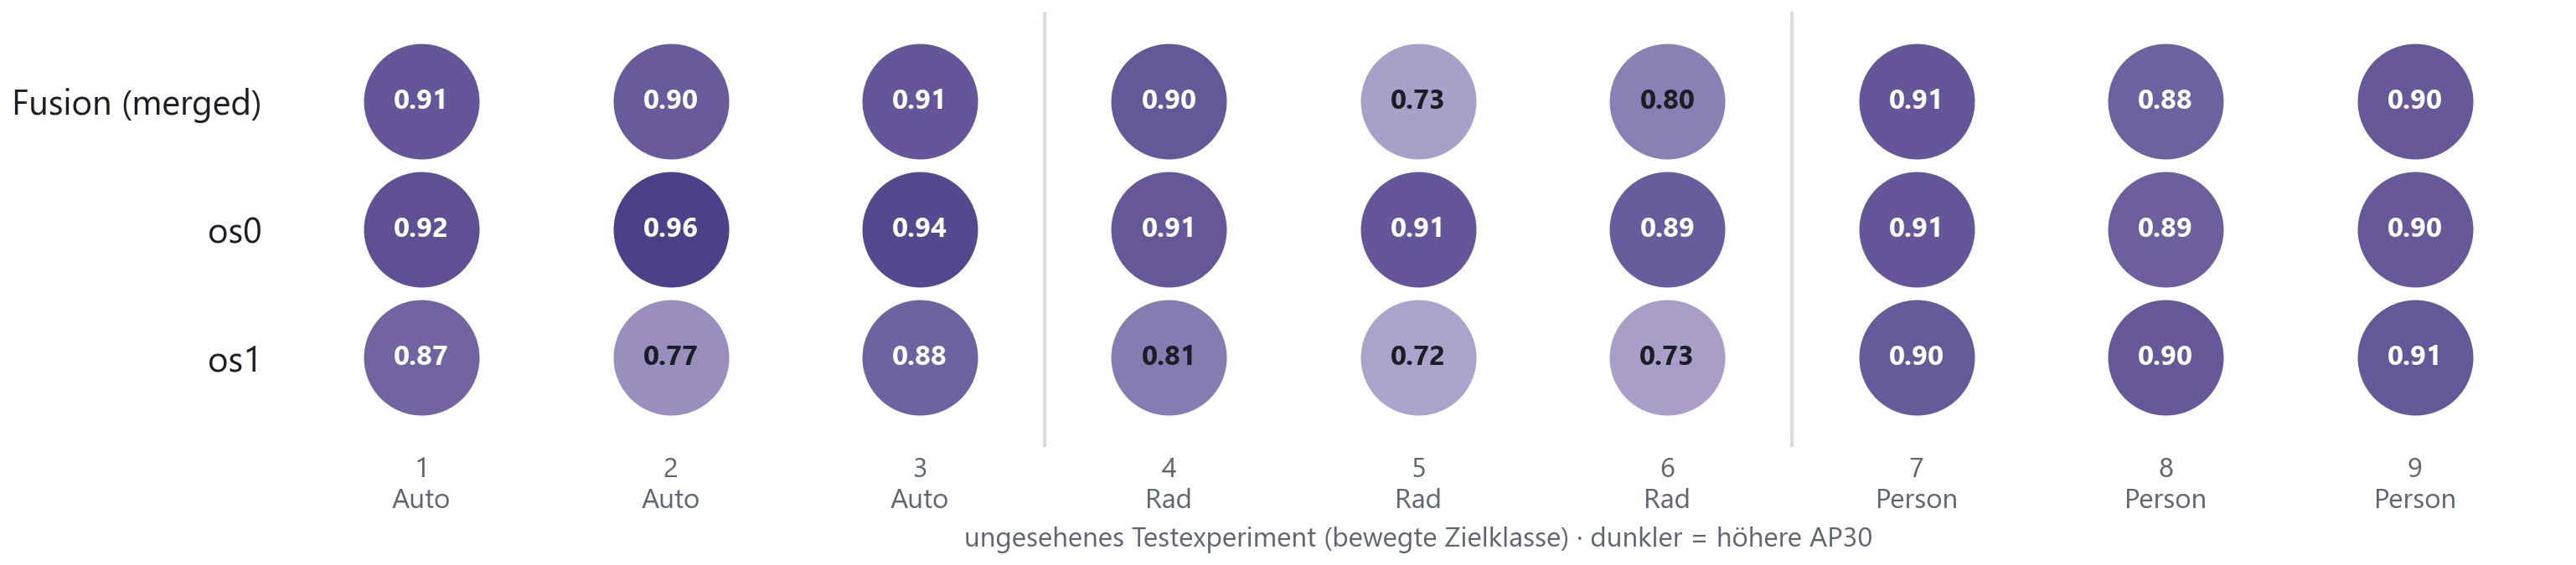
\includegraphics[width=\textwidth]{images/ap30-je-experiment.png}
\caption[AP\textsubscript{30} je ungesehenem Testexperiment]{AP\textsubscript{30} der bewegten Zielklasse je ungesehenem Testexperiment und Ansicht. Jede Spalte wurde von demjenigen Foldmodell vorhergesagt, für das dieses Experiment vollständig ungesehen war.}
\label{fig:ap30-je-experiment}
\end{figure}

Aus dieser Darstellung folgen drei Beobachtungen:

\begin{itemize}
    \item Es gibt keinen Ausfall. Der schlechteste Wert des gesamten Rasters beträgt 0{,}72 (\texttt{os1}, Fahrrad-Experiment 5). Der frühere Extremwert von 0{,}09 für \texttt{os1} auf dem bewegten Auto tritt unter dem Cross-Validation-Protokoll nicht mehr auf und war ein Artefakt des temporalen Splits.
    \item Beim bewegten Auto ist \texttt{os0} in allen drei Experimenten die stärkste Ansicht (0{,}92, 0{,}96 und 0{,}94). Die Fusion ist hier also nicht erforderlich, um das Auto zu finden. In der gepoolten Auswertung über alle Testframes dreht sich diese Ordnung knapp um (\texttt{merged} 0{,}891 gegenüber \texttt{os0} 0{,}885). Der Grund ist derselbe wie bei den Personen: Auch Autovorhersagen außerhalb der Autoaufnahmen gehen in die Rangliste ein. Welche Ansicht das bewegte Auto tatsächlich findet, beantwortet deshalb die experimentweise Auswertung; wie sich die Ansichten über den gesamten Betrieb hinweg verhalten, die gepoolte.
    \item Auf dieser Auswertung ist \texttt{os0} die stärkste und zugleich gleichmäßigste Ansicht. Über alle neun Experimente erreicht \texttt{os0} im Mittel 0{,}914 bei einer Standardabweichung von 0{,}023, \texttt{merged} 0{,}871 bei 0{,}063 und \texttt{os1} 0{,}832 bei 0{,}076. Die Fusion fällt im Fahrrad-Experiment 5 auf 0{,}73 ab und liegt in den Personen-Experimenten 8 und 9 knapp hinter \texttt{os1}.
\end{itemize}

Der letzte Punkt verdient Betonung, weil er der Fusionsthese zunächst widerspricht: Gemessen an der reinen Auffindrate über einzelne Experimente ist die Fusion nicht die beste Ansicht. Das ist kein Widerspruch zu den vorangegangenen Abschnitten, sondern eine Folge dessen, was dieses Raster misst. Es zeigt ausschließlich AP\textsubscript{30}, also die grobe Detektion. Der Vorteil der Fusion liegt nach Abschnitt~\ref{sec:bewegte-klassen} bei den strengeren Schwellen: Dort führt \texttt{merged} in der labelbasierten Auswertung in allen drei Klassen, bei Person und Fahrrad mit erheblichem Abstand. Ein vollständiges Bild ergäbe erst ein entsprechendes Raster für AP\textsubscript{60}, das bislang nicht vorliegt.

Zur Einordnung des Fahrrad-Experiments 5 siehe den folgenden Abschnitt; der dortige Sichtbarkeitseffekt erklärt den Abfall zu einem erheblichen Teil.

\subsection{Warum ist Fahrrad-\texorpdfstring{AP\textsubscript{30}}{AP30} bei os0 höher?}

\texttt{os0} erreicht bei Fahrrädern einen höheren AP\textsubscript{30}, während \texttt{merged} bei AP\textsubscript{60} deutlich führt. Ein Teil des AP\textsubscript{30}-Unterschieds ist ein Sichtbarkeits- und Label-Effekt. Die Ansichten enthalten nicht dieselbe Fahrrad-GT-Menge.

Besonders deutlich ist Experiment 5 (Tabelle~\ref{tab:exp5-bicycle}):

\begin{table}[H]
\centering
\begin{tabular}{ccc}
\toprule
\textbf{Ansicht} & \textbf{Fahrrad-GT} & \textbf{AP\textsubscript{30}} \\
\midrule
merged & 310 & 0{,}727 \\
os0    & 244 & 0{,}907 \\
\bottomrule
\end{tabular}
\caption{Experiment 5: Fahrrad-Ground-Truth-Anzahl und AP\textsubscript{30} nach Ansicht.}
\label{tab:exp5-bicycle}
\end{table}

In den Rohannotationen liegen die zusätzlichen \texttt{merged}-Fahrradframes gegenüber \texttt{os0} überwiegend weiter entfernt. \texttt{os0} wird damit teilweise nur auf dem kürzeren, gut sichtbaren Trajektorienabschnitt bewertet. Eine objektweise vollständig faire Aussage darüber, ob \texttt{merged} dieselben Fahrräder schlechter findet, würde eine zusätzliche Auswertung auf einer gemeinsamen Referenz-GT-Menge erfordern.

Unabhängig davon zeigt AP\textsubscript{60}, dass die von \texttt{merged} gefundenen Fahrräder räumlich wesentlich genauer lokalisiert werden. Die kurze Interpretation lautet daher: \texttt{os0} besitzt in seiner eigenen Labelmenge die vollständigere Groberkennung, die Fusion liefert die präziseren Boxen.

\subsection{Offizielle dynamische Auswertung und \texorpdfstring{AP\textsubscript{60}}{AP60}-Artefakt}
\label{sec:ap60-artefakt}

In der offiziellen dynamischen Auswertung beträgt der Auto-AP\textsubscript{30}/AP\textsubscript{60} \(0{,}877/0{,}739\) für \texttt{merged}, \(0{,}885/0{,}847\) für \texttt{os0} und \(0{,}831/0{,}783\) für \texttt{os1}. Der niedrige offizielle AP\textsubscript{60} von \texttt{merged} entsteht nicht primär durch eine schlechte Box auf dem bewegten Auto. Die beste \texttt{merged}-Box auf dem bewegten Auto hat im Median sogar die höchste IoU der drei Ansichten (\(0{,}848\)).

Der Haupttreiber ist ein nahe am Sensor geparktes Fahrzeug. Zahlreiche hochkonfidente \texttt{merged}-Vorhersagen liegen dort bei IoU 0{,}25--0{,}60. Sie werden bei der offiziellen AP\textsubscript{60}-Teilbewertung nicht mehr als statische Ignore-Treffer erkannt und erscheinen als False Positives in der dynamischen Rangliste. Die labelbasierte Variante ordnet diese Vorhersagen dem statischen Objekt zu; der \texttt{merged}-Auto-AP\textsubscript{60} steigt dadurch von 0{,}739 auf 0{,}883.

\subsection{Vergleich zu CenterPoint}
\label{sec:centerpoint-ergebnis}

Der in Abschnitt~\ref{sec:evalprotokoll} beschriebene Vergleich mit CenterPoint prüft, ob der Fusionsbefund an der gewählten Architektur hängt. Abbildung~\ref{fig:pp-vs-cp} zeigt die Fold-Mittel beider Modelle unter identischem Protokoll.

\begin{figure}[H]
\centering
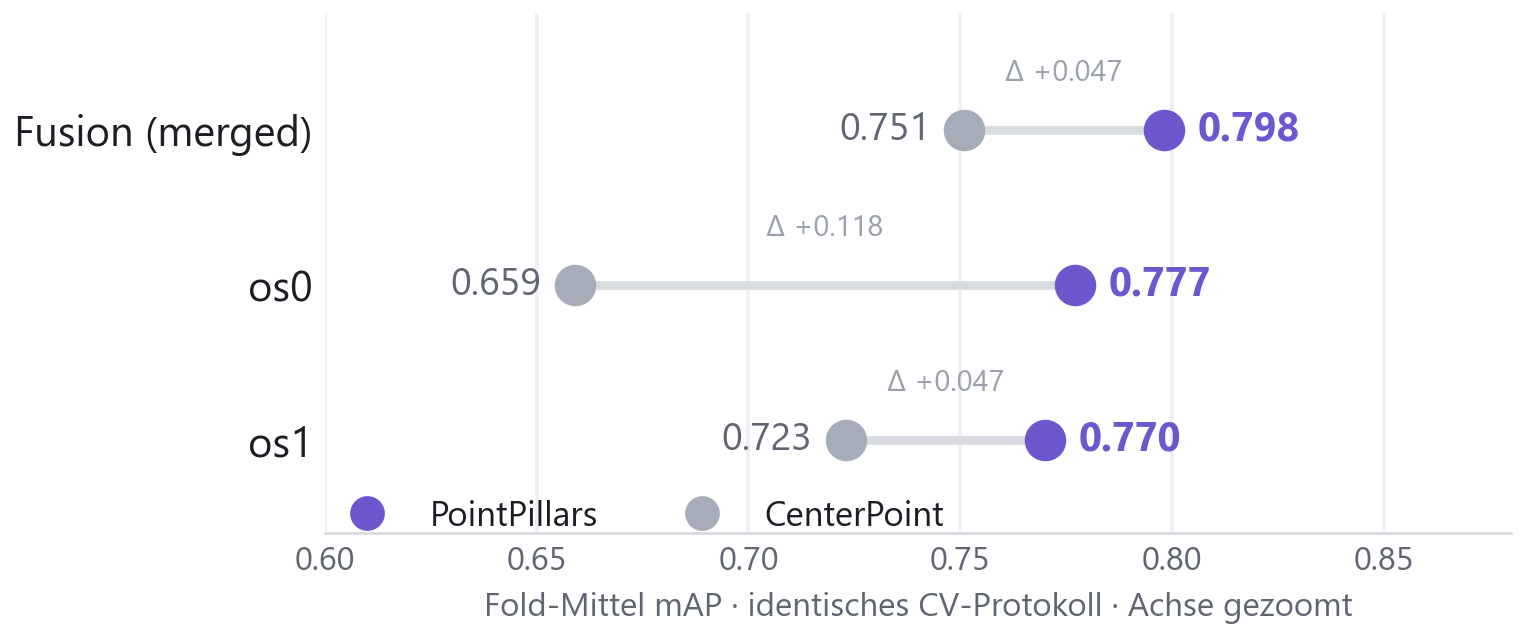
\includegraphics[width=0.9\textwidth]{images/pointpillars-vs-centerpoint.png}
\caption[PointPillars gegenüber CenterPoint]{Gesamt-mAP im Fold-Mittel: PointPillars gegenüber CenterPoint unter identischem Cross-Validation-Protokoll.}
\label{fig:pp-vs-cp}
\end{figure}

Das qualitative Ergebnis ist gegenüber dieser Alternativarchitektur robust: Auch bei CenterPoint ist \texttt{merged} in jedem Fold die beste Ansicht. Mit zwei getesteten Architekturen lässt sich zeigen, dass der Befund nicht ausschließlich an PointPillars hängt; eine allgemeine Architekturunabhängigkeit ist damit nicht belegt, zumal beide Modelle derselben gitterbasierten Detektorfamilie angehören. Die absolute Leistung liegt jedoch in allen drei Ansichten unter PointPillars, mit einem Abstand von 0{,}047 bis 0{,}118 mAP. Der Abstand entsteht vor allem durch die schwächere Lokalisierung von CenterPoint bei strengeren IoU-Schwellen, unter der labelbasierten dynamischen Auswertung besonders deutlich bei Fahrrädern.

Der Fusionsbefund hängt somit nicht an der anchorbasierten PointPillars-Architektur. Zusammen mit dem Ergebnis aus Abschnitt~\ref{sec:finetuning-wirkung} ergibt sich ein konsistentes Bild: Der Unterschied zwischen den Architekturen bewegt sich im Bereich von etwa 0{,}05 bis 0{,}12 mAP, der Unterschied zwischen vortrainiert und finetunet dagegen im Bereich von 0{,}74. Da beide Modelle in Trainingsprotokoll und Datengrundlage übereinstimmen und sich nur in der Architektur und den an sie gebundenen Einstellungen unterscheiden (Abschnitt~\ref{sec:architekturvergleich}), ist dieser Abstand auf den vorliegenden Daten kontrolliert gemessen. Auf eine allgemeine Überlegenheit von PointPillars gegenüber CenterPoint lässt er sich dennoch nicht verallgemeinern: Beide Modelle liefen in ihrer jeweiligen Referenzkonfiguration auf einer einzigen Szene, und ein gezielt auf diese Daten abgestimmtes CenterPoint könnte anders abschneiden. Für die weitere Ergebnisdiskussion bleibt PointPillars das Hauptmodell.
